\documentclass[11pt,a4paper]{article}
% ============================================================
% Packages
% ============================================================
\usepackage[top=3.5cm,bottom=3.5cm,left=3.5cm,right=3.5cm,headheight=14pt]{geometry}
\usepackage{fontspec}
\usepackage{polyglossia}
\setmainlanguage{vietnamese}
\setotherlanguage{english}
\setmainfont{TeX Gyre Termes}
\usepackage{amsmath, amssymb, amsthm}
\usepackage{mathtools}
\usepackage{textcomp}
\usepackage{booktabs}
\usepackage{array}
\usepackage{enumitem}
\usepackage{xcolor}
\usepackage{fancyhdr}
\usepackage{titlesec}
\usepackage{listings}
\usepackage{tikz}
\usetikzlibrary{arrows.meta, positioning}
\usepackage{graphicx}
\graphicspath{{figs/}}
\usepackage{caption}
\captionsetup{font=small}
\usepackage[style=authoryear, backend=biber, maxbibnames=3, maxcitenames=2]{biblatex}
\addbibresource{references.bib}

% ============================================================
% Header / Footer
% ============================================================
\pagestyle{fancy}
\fancyhf{}
\rhead{\small Xử lý số liệu thống kê -- MTT020}
\lhead{\small Master Proba-Stat 2025--2026}
\cfoot{\thepage}

% ============================================================
% Section formatting
% ============================================================
\titleformat{\section}[block]{\large\bfseries\color{blue!70!black}}{}{0em}{}[\titlerule]
\titleformat{\subsection}[runin]{\bfseries}{}{0em}{}[.\ ]

% ============================================================
% Theorem-like environments
% ============================================================
\newtheorem*{baitap}{Bài tập}
\newtheorem*{note}{Lưu ý}

% ============================================================
% Code listings
% ============================================================
\lstset{
  language=Python,
  basicstyle=\small\ttfamily,
  keywordstyle=\color{blue}\bfseries,
  commentstyle=\color{green!50!black},
  stringstyle=\color{orange!80!black},
  numbers=left,
  numberstyle=\tiny\color{gray},
  frame=single,
  breaklines=true,
  tabsize=4,
  showstringspaces=false,
  xleftmargin=1.5em,
}

% Pseudocode listing style
\lstdefinestyle{pseudo}{
  language={},
  basicstyle=\small\ttfamily,
  keywordstyle=\bfseries,
  morekeywords={for, each, if, then, else, return, end, while, do, Input, Output, function},
  numbers=left,
  numberstyle=\tiny\color{gray},
  frame=single,
  breaklines=true,
  tabsize=2,
  xleftmargin=1.5em,
  commentstyle=\color{green!50!black}\itshape,
  morecomment=[l]{//},
}

% ============================================================
% Shortcuts
% ============================================================
\newcommand{\E}{\mathbb{E}}
\newcommand{\Var}{\operatorname{Var}}
\newcommand{\Prob}{\mathbb{P}}
\newcommand{\Z}{\mathbb{Z}}
\newcommand{\N}{\mathbb{N}}
\newcommand{\R}{\mathbb{R}}
\newcommand{\MAD}{\operatorname{MAD}}
\newcommand{\lrd}{\operatorname{lrd}}
\newcommand{\LOF}{\operatorname{LOF}}

% ============================================================
\begin{document}
% ============================================================

\begin{center}
  {\LARGE\bfseries BÀI TẬP NHÓM SỐ 1: XÁC ĐỊNH ĐIỂM NGOẠI LAI}\\[0.5em]
  {\large XỬ LÝ SỐ LIỆU THỐNG KÊ -- MTT020 \\[0.3em]}
\end{center}

\begin{center}
\begin{tabular}{ l c }
\textbf{Họ và tên} & \textbf{Mã học viên} \\ \hline \\
LÊ HOÀNG NHƯ & 25C23014 \\
PHẠM ĐOÀN VỊNH NGHI & 25C23 \\
NGUYỄN NHẬT QUANG & 25C23 \\
\end{tabular}
\end{center}

\begin{center}
  \textit{Tháng 5, 2026}
\end{center}

\vspace{1em}
\hrule
\vspace{1.5em}

% ============================================================
\section{Giới thiệu}
% ============================================================

Trong thực tế phân tích dữ liệu, không phải mọi quan sát đều tuân theo cùng một cơ chế sinh dữ liệu.
Một số điểm dữ liệu có thể xuất hiện do lỗi đo lường, sự cố hệ thống, hoặc chính xác là các sự kiện bất thường cần được phát hiện.
\textcite{hawkins1980} định nghĩa điểm ngoại lai (outlier) như sau:

\begin{quote}
  \textit{``An outlier is an observation which deviates so much from the other observations as to arouse suspicions that it was generated by a different mechanism.''}
\end{quote}

\subsection{Phân loại điểm ngoại lai}
\textcite{chandola2009} phân loại điểm ngoại lai thành ba loại chính:

\begin{enumerate}[noitemsep]
  \item \textbf{Điểm ngoại lai toàn cục (Point outlier):} Một quan sát đơn lẻ lệch rõ ràng so với phần còn lại của tập dữ liệu. Đây là dạng phổ biến nhất và đơn giản nhất để phát hiện.
  \item \textbf{Điểm ngoại lai ngữ cảnh (Contextual outlier):} Một quan sát chỉ bất thường trong một ngữ cảnh nhất định (ví dụ: nhiệt độ 35°C là bình thường vào mùa hè nhưng bất thường vào mùa đông).
  \item \textbf{Điểm ngoại lai tập thể (Collective outlier):} Một tập hợp các quan sát cùng nhau tạo thành bất thường dù mỗi quan sát đơn lẻ có thể bình thường (ví dụ: một chuỗi thời gian lặp lại bất thường).
\end{enumerate}

\subsection{Tầm quan trọng trong thực tiễn}
Phát hiện điểm ngoại lai có ứng dụng rộng rãi trong công nghiệp:
gian lận tài chính (phát hiện giao dịch đáng ngờ), kiểm soát chất lượng sản xuất (phát hiện sản phẩm lỗi),
an ninh mạng (phát hiện xâm nhập), chăm sóc sức khỏe (phát hiện kết quả xét nghiệm bất thường),
và giám sát thiết bị IoT (phát hiện lỗi cảm biến).

% ============================================================
\section{Phương pháp thống kê cổ điển (Đơn biến)}
% ============================================================

Các phương pháp đơn biến xem xét từng thuộc tính độc lập và phù hợp khi dữ liệu có ít chiều hoặc khi cần một phương pháp nhanh, dễ giải thích.

% --------------------------------------------------
\subsection{Z-score (Điểm chuẩn hóa)}

\textbf{Ý tưởng.} Chuẩn hóa mỗi quan sát theo trung bình và độ lệch chuẩn mẫu, sau đó đặt ngưỡng dựa trên phân phối chuẩn.

\textbf{Công thức.} Với tập dữ liệu $\{x_1, \ldots, x_n\}$, Z-score của quan sát $x_i$ là:
\begin{equation}
  z_i = \frac{x_i - \bar{x}}{s}, \quad
  \bar{x} = \frac{1}{n}\sum_{i=1}^n x_i, \quad
  s = \sqrt{\frac{1}{n-1}\sum_{i=1}^n (x_i - \bar{x})^2}.
\end{equation}

\textbf{Quy tắc phán quyết.} Quan sát $x_i$ được coi là ngoại lai nếu $|z_i| > 3$.
Dưới phân phối chuẩn, $\Prob(|Z| > 3) \approx 0{,}27\%$, nên ngưỡng này tương ứng với mức ý nghĩa thực tế rất nhỏ.

\textbf{Ưu điểm:} đơn giản, nhanh, dễ giải thích.\\
\textbf{Nhược điểm:} giả định phân phối Gaussian; bị ảnh hưởng bởi chính các điểm ngoại lai (masking effect); không hiệu quả với phân phối đuôi nặng.

\begin{lstlisting}[style=pseudo, caption={Thuật toán Z-score}, label={lst:zscore}]
Input:  data x[1..n], threshold tau = 3
Output: outliers O

mean = average(x)
std  = standard_deviation(x)
O = []
for each x_i in x:
    z_i = (x_i - mean) / std
    if |z_i| > tau then
        O.append(x_i)
return O
\end{lstlisting}

\noindent\textbf{Minh họa thực nghiệm.}
\begin{center}
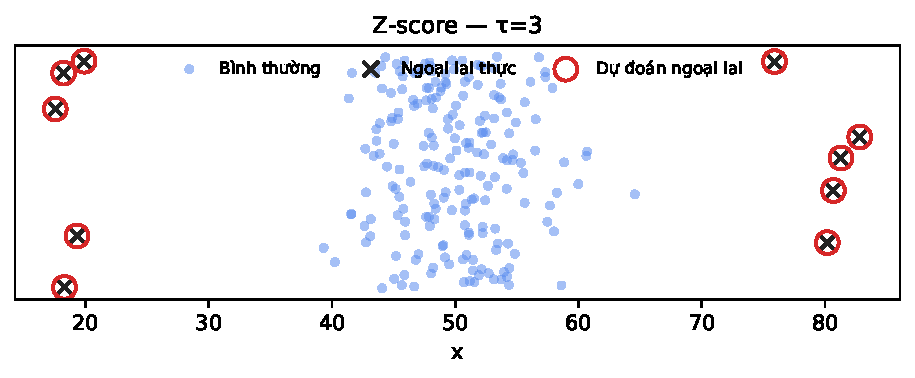
\includegraphics[width=0.72\textwidth]{zscore.pdf}
\end{center}
\noindent Trên dataset UD ($n = 210$, 10 ngoại lai thực): phát hiện $10/10$ ngoại lai, không có dương tính giả; $F_1 = 1{,}000$, AUC $= 1{,}000$.

% --------------------------------------------------
\subsection{Modified Z-score (Iglewicz \& Hoaglin)}

\textbf{Ý tưởng.} Thay thế trung bình và độ lệch chuẩn bằng các ước lượng robust hơn: trung vị $\tilde{x}$ và độ lệch tuyệt đối trung vị (\textit{Median Absolute Deviation}, MAD) \parencite{iglewicz1993}.

\textbf{Công thức.}
\begin{equation}
  \MAD = \text{median}\bigl(|x_i - \tilde{x}|\bigr), \qquad
  M_i = \frac{0{,}6745\,(x_i - \tilde{x})}{\MAD}.
\end{equation}
Hệ số $0{,}6745 = \Phi^{-1}(3/4)$ được chọn để $\MAD / 0{,}6745$ là ước lượng nhất quán của $\sigma$ dưới phân phối chuẩn.

\textbf{Quy tắc phán quyết.} Quan sát $x_i$ là ngoại lai nếu $|M_i| > 3{,}5$.

\textbf{Ưu điểm:} robust -- ngay cả khi có nhiều điểm ngoại lai trong dữ liệu, ước lượng $\tilde{x}$ và $\MAD$ vẫn ổn định. Breakdown point đạt 50\%.

\begin{lstlisting}[style=pseudo, caption={Modified Z-score}, label={lst:modz}]
Input:  data x[1..n], threshold tau = 3.5
Output: outliers O

x_med = median(x)
MAD   = median(|x_i - x_med| for each x_i in x)
O = []
for each x_i in x:
    M_i = 0.6745 * (x_i - x_med) / MAD
    if |M_i| > tau then
        O.append(x_i)
return O
\end{lstlisting}

\noindent\textbf{Minh họa thực nghiệm.}
\begin{center}
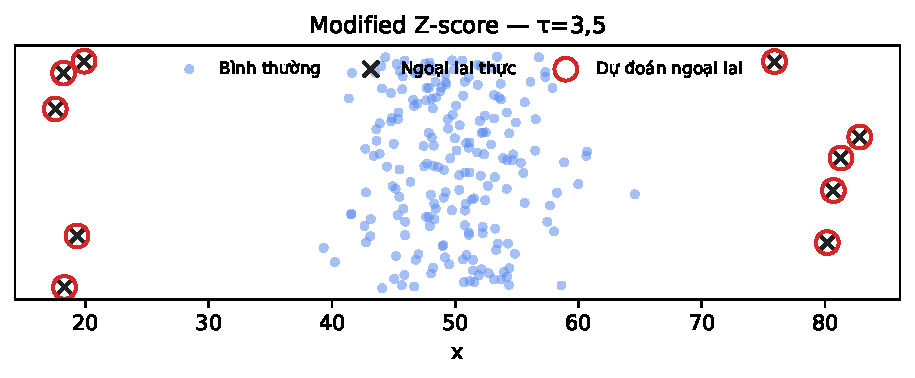
\includegraphics[width=0.72\textwidth]{modz.pdf}
\end{center}
\noindent Trên dataset UD: phát hiện $10/10$ ngoại lai, không có dương tính giả; $F_1 = 1{,}000$, AUC $= 1{,}000$. Kết quả khẳng định robustness của ước lượng dựa trên trung vị và MAD.

% --------------------------------------------------
\subsection{Phương pháp IQR (Tukey's Fences)}

\textbf{Ý tưởng.} Sử dụng tứ phân vị để xác định vùng bình thường, không giả định phân phối \parencite{tukey1977}.

\textbf{Công thức.}
\begin{equation}
  \text{IQR} = Q_3 - Q_1,
\end{equation}
với $Q_1$, $Q_3$ lần lượt là tứ phân vị thứ nhất và thứ ba.

\textbf{Quy tắc phán quyết.} Hai cặp hàng rào được định nghĩa:
\begin{align}
  \text{Hàng rào trong:} &\quad L_{\text{in}} = Q_1 - 1{,}5\cdot\text{IQR}, \quad U_{\text{in}} = Q_3 + 1{,}5\cdot\text{IQR}; \\
  \text{Hàng rào ngoài:} &\quad L_{\text{out}} = Q_1 - 3\cdot\text{IQR}, \quad U_{\text{out}} = Q_3 + 3\cdot\text{IQR}.
\end{align}
Điểm nằm ngoài hàng rào trong được coi là \textit{nghi ngờ ngoại lai}; điểm nằm ngoài hàng rào ngoài là \textit{ngoại lai cực đoan}.

\textbf{Ưu điểm:} không tham số, đây là nền tảng của biểu đồ hộp (\textit{box plot}) và được sử dụng phổ biến trong phân tích dữ liệu khám phá (EDA).

\begin{lstlisting}[style=pseudo, caption={Phương pháp IQR (Tukey's Fences)}, label={lst:iqr}]
Input:  data x[1..n], k_inner = 1.5, k_outer = 3.0
Output: suspected outliers O_in, extreme outliers O_out

Q1, Q3 = quartiles(x)
IQR = Q3 - Q1
L_in  = Q1 - k_inner * IQR;  U_in  = Q3 + k_inner * IQR
L_out = Q1 - k_outer * IQR;  U_out = Q3 + k_outer * IQR
O_in  = {x_i : x_i < L_in  or x_i > U_in}
O_out = {x_i : x_i < L_out or x_i > U_out}
return O_in, O_out
\end{lstlisting}

\noindent\textbf{Minh họa thực nghiệm.}
\begin{center}
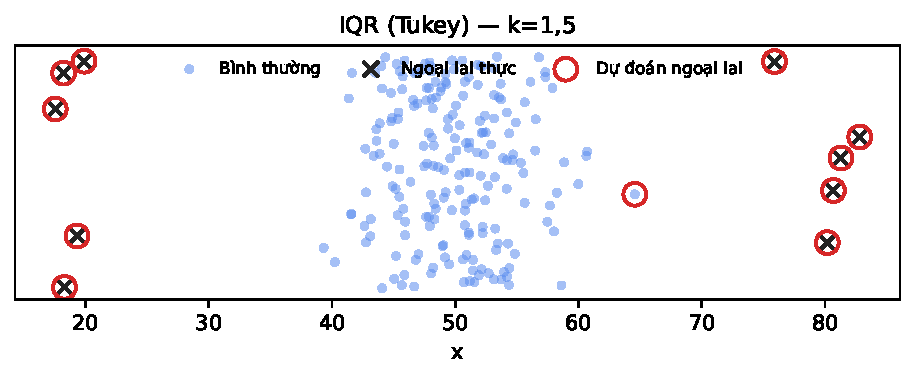
\includegraphics[width=0.72\textwidth]{iqr.pdf}
\end{center}
\noindent Trên dataset UD: phát hiện $11$ điểm trong đó $10/10$ là ngoại lai thực và $1$ dương tính giả nằm ngay rìa hàng rào trong; $F_1 = 0{,}952$, AUC $= 1{,}000$. Đây là biểu hiện tự nhiên của hệ số $1{,}5$ — một số quan sát đuôi nhẹ của phân phối nội tại bị xếp vào nhóm ``nghi ngờ''.

% --------------------------------------------------
\subsection{Kiểm định Grubbs}

\textbf{Ý tưởng.} Kiểm định thống kê chính thức cho giả thuyết ``không có điểm ngoại lai'' trong mẫu Gaussian \parencite{grubbs1969}.

\textbf{Thống kê kiểm định.}
\begin{equation}
  G = \frac{\max_{i}\,|x_i - \bar{x}|}{s}.
\end{equation}

\textbf{Giá trị tới hạn.} Dưới $H_0$: dữ liệu đến từ phân phối chuẩn và không có ngoại lai,
\begin{equation}
  G_{\text{crit}} = \frac{n-1}{\sqrt{n}}\sqrt{\frac{t^2_{\alpha/(2n),\,n-2}}{n - 2 + t^2_{\alpha/(2n),\,n-2}}},
\end{equation}
với $t_{\alpha/(2n),\,n-2}$ là phân vị $\alpha/(2n)$ của phân phối Student $t$ với $n-2$ bậc tự do.
Bác bỏ $H_0$ nếu $G > G_{\text{crit}}$.

\textbf{Phát hiện nhiều ngoại lai (ESD).} Áp dụng kiểm định Grubbs lặp lại: sau mỗi bước, loại bỏ quan sát cực trị nhất rồi kiểm định lại trên mẫu thu nhỏ, cho đến khi không còn ngoại lai hoặc đạt số lượng tối đa đã định.

\begin{lstlisting}[style=pseudo, caption={Kiểm định Grubbs / ESD lặp}, label={lst:grubbs}]
Input:  data x[1..n], significance alpha, max_outliers r_max
Output: outliers O

O = []
for r = 1 to r_max:
    mean_x = average(x);  s_x = std(x)
    i_star = argmax(|x_i - mean_x|)
    G = |x[i_star] - mean_x| / s_x
    G_crit = (n-1)/sqrt(n) * sqrt(t2 / (n-2+t2))
        // t2 = t_quantile(alpha/(2*n), df=n-2)^2
    if G <= G_crit then break   // stop: no more outliers
    O.append(x[i_star])
    x.remove(i_star);  n = n - 1
return O
\end{lstlisting}

\noindent\textbf{Minh họa thực nghiệm.}
\begin{center}
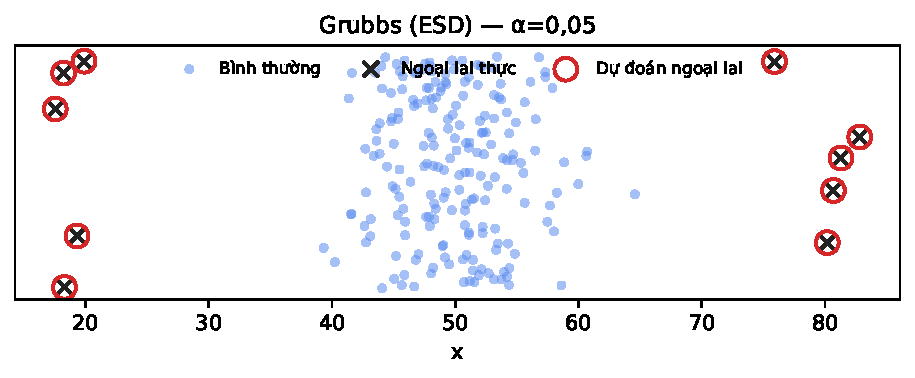
\includegraphics[width=0.72\textwidth]{grubbs.pdf}
\end{center}
\noindent Trên dataset UD ($\alpha = 0{,}05$, lặp tối đa 15 vòng): kiểm định ESD dừng đúng tại $r^\star = 10$, phát hiện $10/10$ ngoại lai thực; $F_1 = 1{,}000$, AUC $= 1{,}000$.

% ============================================================
\section{Phương pháp đa biến}
% ============================================================

Khi dữ liệu có nhiều chiều và các biến tương quan với nhau, các phương pháp đơn biến áp dụng độc lập cho từng chiều có thể bỏ sót những điểm bất thường chỉ xuất hiện trong không gian kết hợp.

% --------------------------------------------------
\subsection{Khoảng cách Mahalanobis}

\textbf{Ý tưởng.} Đo khoảng cách của một điểm so với tâm của phân phối, có tính đến hướng và độ tản mạn của dữ liệu \parencite{mahalanobis1936}.

\textbf{Công thức.} Với vector quan sát $\mathbf{x} \in \R^p$, trung bình $\boldsymbol{\mu}$ và ma trận hiệp phương sai $\boldsymbol{\Sigma}$:
\begin{equation}
  D^2(\mathbf{x}) = (\mathbf{x} - \boldsymbol{\mu})^\top \boldsymbol{\Sigma}^{-1} (\mathbf{x} - \boldsymbol{\mu}).
\end{equation}

Trong thực tế, $\boldsymbol{\mu}$ và $\boldsymbol{\Sigma}$ được ước lượng bằng trung bình mẫu $\bar{\mathbf{x}}$ và ma trận hiệp phương sai mẫu $\mathbf{S}$.

\textbf{Phân phối.} Nếu dữ liệu tuân theo $\mathcal{N}_p(\boldsymbol{\mu}, \boldsymbol{\Sigma})$ thì $D^2 \sim \chi^2(p)$.

\textbf{Quy tắc phán quyết.} Quan sát $\mathbf{x}_i$ là ngoại lai nếu:
\begin{equation}
  D^2(\mathbf{x}_i) > \chi^2_{\alpha,\,p},
\end{equation}
với $\chi^2_{\alpha,p}$ là phân vị $(1-\alpha)$ của phân phối chi-bình phương $p$ bậc tự do, thường chọn $\alpha = 0{,}05$.

\textbf{Hạn chế và cải tiến.} Ma trận hiệp phương sai mẫu $\mathbf{S}$ nhạy cảm với chính các điểm ngoại lai.
Phương pháp \textit{Minimum Covariance Determinant} (MCD) \parencite{rousseeuw1999} ước lượng $\boldsymbol{\Sigma}$ bằng cách tìm tập $h$ quan sát (thường $h \approx 0{,}75n$) có hiệp phương sai nhỏ nhất, cho ước lượng robust hơn.

\begin{lstlisting}[style=pseudo, caption={Khoảng cách Mahalanobis}, label={lst:mahal}]
Input:  data X[n x p], significance level alpha
Output: outliers O

x_bar = column_mean(X)
S = sample_covariance(X)
S_inv = inverse(S)
O = []
for each x_i in X:
    d2 = (x_i - x_bar)' * S_inv * (x_i - x_bar)
    if d2 > chi2_quantile(1 - alpha, df = p) then
        O.append(x_i)
return O
\end{lstlisting}

\noindent\textbf{Minh họa thực nghiệm.}
\begin{center}
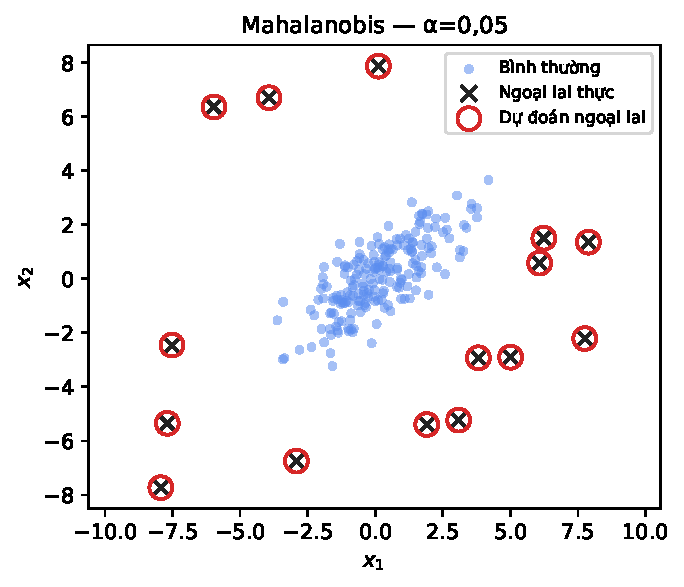
\includegraphics[width=0.55\textwidth]{mahalanobis.pdf}
\end{center}
\noindent Trên dataset MD2 ($n = 215$, 15 ngoại lai uniform xa khỏi cụm Gaussian tương quan): phát hiện $15/15$ với $\alpha = 0{,}05$, không có dương tính giả; $F_1 = 1{,}000$, AUC $= 1{,}000$. Khoảng cách Mahalanobis tính đến hướng tương quan của $\mathbf{S}$ nên các điểm chỉ ``hơi xa trục dài'' vẫn được xác định chính xác.

% --------------------------------------------------
\subsection{Phát hiện ngoại lai dựa trên PCA}

\textbf{Ý tưởng.} Chiếu dữ liệu lên không gian các thành phần chính và phân tích hai nguồn biến động: biến động \textit{bên trong} mô hình (T²) và biến động \textit{bên ngoài} mô hình (thống kê Q) \parencite{jackson1979}.

\textbf{Phân tích.} Giả sử đã chọn $k$ thành phần chính với ma trận tải $\mathbf{P}_k \in \R^{p \times k}$ và ma trận trị riêng $\boldsymbol{\Lambda}_k = \mathrm{diag}(\lambda_1, \ldots, \lambda_k)$. Điểm số của $\mathbf{x}$ trong không gian PC là:
\begin{equation}
  \mathbf{t} = \mathbf{P}_k^\top (\mathbf{x} - \bar{\mathbf{x}}).
\end{equation}

\textbf{Thống kê Hotelling T².} Đo độ lệch trong không gian mô hình:
\begin{equation}
  T^2 = \mathbf{t}^\top \boldsymbol{\Lambda}_k^{-1} \mathbf{t}.
\end{equation}

\textbf{Thống kê Q (SPE --- Squared Prediction Error).} Đo sai số tái tạo (phần biến động không được giải thích bởi $k$ thành phần):
\begin{equation}
  Q = \|\mathbf{x} - \bar{\mathbf{x}} - \mathbf{P}_k \mathbf{t}\|^2 = \|(\mathbf{I} - \mathbf{P}_k\mathbf{P}_k^\top)(\mathbf{x} - \bar{\mathbf{x}})\|^2.
\end{equation}

\textbf{Quy tắc phán quyết.} Quan sát $\mathbf{x}_i$ là ngoại lai nếu $T^2 > T^2_{\text{crit}}$ hoặc $Q > Q_{\text{crit}}$.
Giá trị tới hạn $Q_{\text{crit}}$ được tính theo công thức Jackson--Mudholkar sử dụng các trị riêng còn lại $\lambda_{k+1}, \ldots, \lambda_p$.

\begin{note}
  T² cao nhưng Q thấp: điểm bất thường trong không gian PC, vẫn nằm trong mô hình.
  Q cao: điểm nằm ngoài không gian mô hình hoàn toàn --- thường là ngoại lai thực sự.
\end{note}

\begin{lstlisting}[style=pseudo, caption={Phát hiện ngoại lai bằng PCA (T² và Q)}, label={lst:pca}]
Input:  data X[n x p], num_components k, alpha
Output: outliers O

X_c = X - column_mean(X)              // center data
[P, Lambda] = top_k_PCA(X_c, k)      // loadings P[p x k], eigenvalues Lambda
T2_crit = chi2_quantile(1-alpha, df=k)
Q_crit  = jackson_mudholkar_ucl(all_eigenvalues, k, alpha)

O = []
for each x in X:
    t  = P' * (x - mean(X))           // scores in PC space
    T2 = t' * inv(Lambda) * t
    Q  = norm((I - P*P') * (x - mean(X)))^2
    if T2 > T2_crit or Q > Q_crit then
        O.append(x)
return O
\end{lstlisting}

\noindent\textbf{Minh họa thực nghiệm.}
\begin{center}
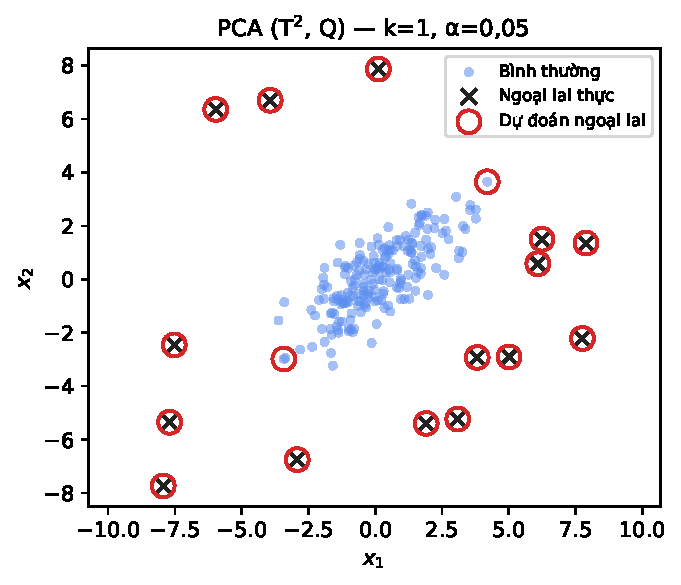
\includegraphics[width=0.55\textwidth]{pca.pdf}
\end{center}
\noindent Trên dataset MD2 ($k = 1$ thành phần chính giải thích $71{,}3\%$ phương sai, $\alpha = 0{,}05$): kết hợp $T^2$ và $Q$ phát hiện $15/15$ ngoại lai kèm $2$ dương tính giả; $F_1 = 0{,}938$, AUC $= 1{,}000$. Vì dữ liệu chỉ có hai chiều, $Q$ tương đương với khoảng cách vuông góc tới trục PC1 và đóng vai trò chính trong phán quyết.

% ============================================================
\section{Phương pháp dựa trên mật độ}
% ============================================================

Các phương pháp dựa trên mật độ không giả định phân phối toàn cục mà xem xét mật độ cục bộ xung quanh mỗi điểm. Điểm nằm trong vùng thưa hơn các lân cận của nó được coi là ngoại lai.

% --------------------------------------------------
\subsection{DBSCAN}

\textbf{Ý tưởng.} Phân cụm dựa trên mật độ; các điểm không thuộc cụm nào được đánh dấu là noise point và coi là ngoại lai \parencite{ester1996}.

\textbf{Tham số.} $\varepsilon$ (bán kính lân cận) và $\mathit{MinPts}$ (số điểm tối thiểu để tạo thành vùng mật độ cao).

\textbf{Định nghĩa.} Cho lân cận $\varepsilon$-ball của điểm $p$:
\begin{equation}
  N_\varepsilon(p) = \{q \in D : d(p, q) \le \varepsilon\}.
\end{equation}
\begin{itemize}[noitemsep]
  \item \textbf{Core point:} $|N_\varepsilon(p)| \ge \mathit{MinPts}$.
  \item \textbf{Border point:} $|N_\varepsilon(p)| < \mathit{MinPts}$ nhưng $p \in N_\varepsilon(q)$ với một core point $q$.
  \item \textbf{Noise point (outlier):} không phải core point cũng không phải border point.
\end{itemize}

\begin{lstlisting}[style=pseudo, caption={DBSCAN}, label={lst:dbscan}]
Input:  data D, epsilon, MinPts
Output: cluster labels C[], noise set O

C = array of UNVISITED for all points
cluster_id = 0
for each point p in D:
    if C[p] != UNVISITED then continue
    N = range_query(D, p, epsilon)
    if |N| < MinPts then
        C[p] = NOISE
    else:
        cluster_id++
        expand_cluster(p, N, cluster_id, epsilon, MinPts)
O = {p : C[p] == NOISE}
return C, O

function expand_cluster(p, N, id, eps, MinPts):
    C[p] = id
    for each q in N:
        if C[q] == UNVISITED then
            C[q] = id
            N' = range_query(D, q, eps)
            if |N'| >= MinPts then N = N + N'
        if C[q] == NOISE then C[q] = id
\end{lstlisting}

\textbf{Lưu ý.} DBSCAN cho kết quả nhị phân (ngoại lai / không ngoại lai) và không tạo ra điểm số liên tục. Việc chọn $\varepsilon$ thường dựa trên đồ thị k-distance.

\noindent\textbf{Minh họa thực nghiệm.}
\begin{center}
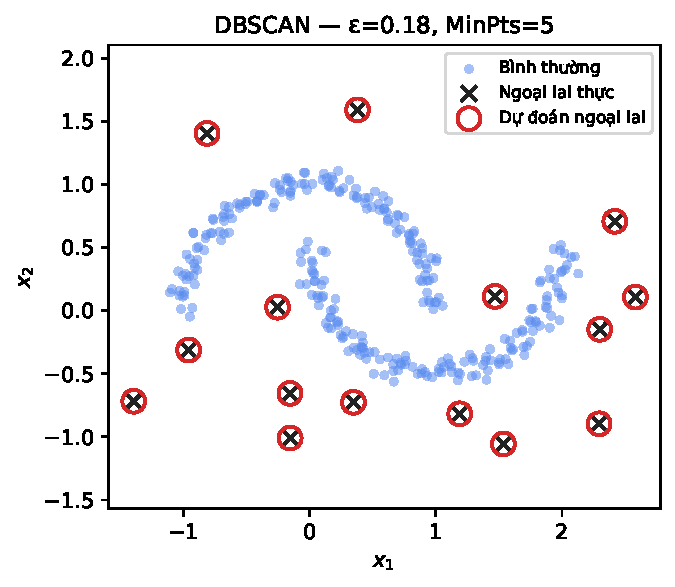
\includegraphics[width=0.55\textwidth]{dbscan.pdf}
\end{center}
\noindent Trên dataset MD-NL (hai cụm half-moon $+ 15$ ngoại lai uniform), chọn $\varepsilon$ tại phân vị 95 của khoảng cách 5-NN cho $\varepsilon \approx 0{,}18$ và MinPts $= 5$: phát hiện $15/15$ ngoại lai, không có dương tính giả; $F_1 = 1{,}000$. AUC dùng khoảng cách 5-NN trung bình làm điểm số đạt $1{,}000$.

% --------------------------------------------------
\subsection{Local Outlier Factor (LOF)}

\textbf{Ý tưởng.} So sánh mật độ cục bộ của một điểm với mật độ cục bộ của các lân cận của nó. Điểm nằm trong vùng thưa hơn đáng kể so với lân cận được gán điểm LOF cao \parencite{breunig2000}.

\textbf{Định nghĩa.} Với $k$ lân cận gần nhất ($k$-NN):

\textit{Khoảng cách khả năng tiếp cận (reachability distance):}
\begin{equation}
  \mathrm{reach\text{-}dist}_k(p, o) = \max\bigl(k\text{-}d(o),\, d(p, o)\bigr),
\end{equation}
với $k$-$d(o)$ là khoảng cách từ $o$ đến lân cận thứ $k$ của nó.

\textit{Mật độ khả năng tiếp cận cục bộ (local reachability density):}
\begin{equation}
  \lrd_k(p) = \frac{|N_k(p)|}{\displaystyle\sum_{o \in N_k(p)} \mathrm{reach\text{-}dist}_k(p, o)}.
\end{equation}

\textit{Chỉ số ngoại lai cục bộ (LOF):}
\begin{equation}
  \LOF_k(p) = \frac{1}{|N_k(p)|}\sum_{o \in N_k(p)} \frac{\lrd_k(o)}{\lrd_k(p)}.
\end{equation}

\textbf{Giải thích.}
$\LOF_k(p) \approx 1$: điểm $p$ có mật độ tương đương lân cận (điểm bình thường).
$\LOF_k(p) \gg 1$: điểm $p$ nằm trong vùng thưa hơn đáng kể so với lân cận (ngoại lai).

\begin{lstlisting}[style=pseudo, caption={Local Outlier Factor}, label={lst:lof}]
Input:  data D, k (number of neighbors), threshold tau
Output: LOF scores, outliers O

for each p in D:
    N_k(p) = k_nearest_neighbors(D, p)
    k_dist(p) = distance(p, N_k(p)[k])  // k-th neighbor distance

for each p in D:
    lrd(p) = |N_k(p)| / sum(reach_dist(p, o) for o in N_k(p))
        where reach_dist(p, o) = max(k_dist(o), d(p, o))

for each p in D:
    LOF(p) = mean(lrd(o) / lrd(p) for o in N_k(p))

O = {p : LOF(p) > tau}
return LOF scores, O
\end{lstlisting}

\noindent\textbf{Minh họa thực nghiệm.}
\begin{center}
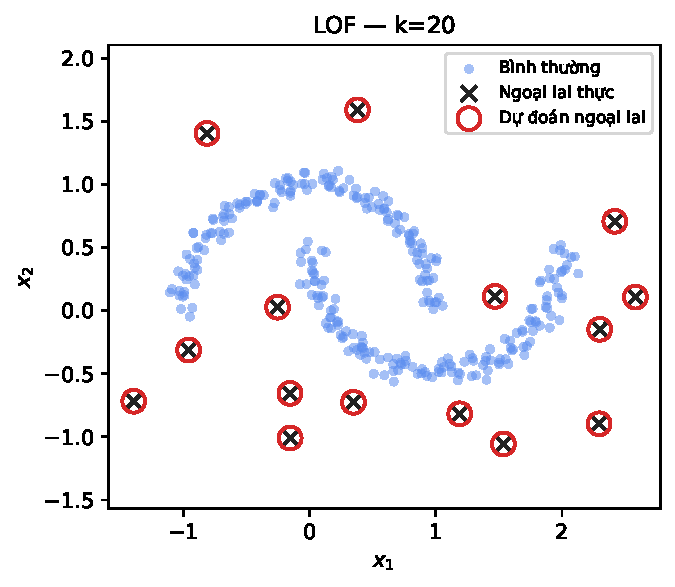
\includegraphics[width=0.55\textwidth]{lof.pdf}
\end{center}
\noindent Trên dataset MD-NL với $k = 20$ và contamination $\approx 4{,}8\%$: phát hiện $15/15$ ngoại lai, không có dương tính giả; $F_1 = 1{,}000$, AUC $= 1{,}000$. Nhờ so sánh \emph{tỉ lệ} mật độ với lân cận, LOF không bị ràng buộc bởi hình dạng của cụm bình thường, một ưu thế rõ rệt so với Mahalanobis trên dữ liệu phi tuyến.

% ============================================================
\section{Phương pháp học máy}
% ============================================================

Các phương pháp học máy không đòi hỏi giả định phân phối và xử lý hiệu quả dữ liệu chiều cao và phi tuyến.

% --------------------------------------------------
\subsection{Isolation Forest}

\textbf{Ý tưởng.} Điểm ngoại lai là các điểm \textit{dễ bị cô lập} hơn so với điểm bình thường \parencite{liu2008}. Xây dựng các cây quyết định ngẫu nhiên (isolation trees) và đo độ sâu trung bình cần thiết để cô lập một điểm.

\textbf{Cây cô lập (iTree).} Mỗi cây được xây dựng bằng cách chọn ngẫu nhiên:
\begin{enumerate}[noitemsep]
  \item Một feature $f$.
  \item Một giá trị tách $v$ đồng đều trong $[\min(f), \max(f)]$.
\end{enumerate}
Điểm $\mathbf{x}$ được cô lập ở lá. Độ sâu $h(\mathbf{x})$ là số cạnh từ gốc đến lá.

\textbf{Anomaly score.} Với $t$ cây và $n$ điểm dữ liệu:
\begin{equation}
  s(\mathbf{x}, n) = 2^{-\,\E[h(\mathbf{x})]\,/\,c(n)},
\end{equation}
với $c(n) = 2H(n-1) - 2(n-1)/n$ là độ sâu trung bình trong cây tìm kiếm nhị phân ($H$ là số điều hòa).

\textbf{Giải thích điểm số:}
\begin{itemize}[noitemsep]
  \item $s \to 1$: đường đi ngắn, dễ cô lập $\Rightarrow$ ngoại lai.
  \item $s \approx 0{,}5$: không rõ ràng.
  \item $s \to 0$: đường đi dài, khó cô lập $\Rightarrow$ điểm bình thường.
\end{itemize}

\begin{lstlisting}[style=pseudo, caption={Isolation Forest}, label={lst:iforest}]
Input:  data X[n x p], n_trees t, subsample size psi, threshold s_min
Output: anomaly scores S[], outliers O

// Training phase
forest = []
for i = 1 to t:
    X_sub = random_sample(X, size=psi)  // subsample without replacement
    tree = build_iTree(X_sub, height_limit = ceil(log2(psi)))
    forest.append(tree)

// Scoring phase
for each x in X:
    h_avg = mean(path_length(x, tree) for tree in forest)
    S[x] = 2^(-h_avg / c(psi))

O = {x : S[x] > s_min}   // s_min typically 0.6
return S, O

function build_iTree(X, height_limit):
    if |X| <= 1 or current_height >= height_limit then return Leaf(size=|X|)
    f = random_feature()
    v = random_uniform(min(X[f]), max(X[f]))
    X_left  = {x in X : x[f] < v}
    X_right = {x in X : x[f] >= v}
    return Node(f, v, build_iTree(X_left, h+1), build_iTree(X_right, h+1))
\end{lstlisting}

\textbf{Ưu điểm:} độ phức tạp tuyến tính $O(t \cdot \psi \log \psi)$, hiệu quả với dữ liệu lớn, không cần tính khoảng cách.

\noindent\textbf{Minh họa thực nghiệm.}
\begin{center}
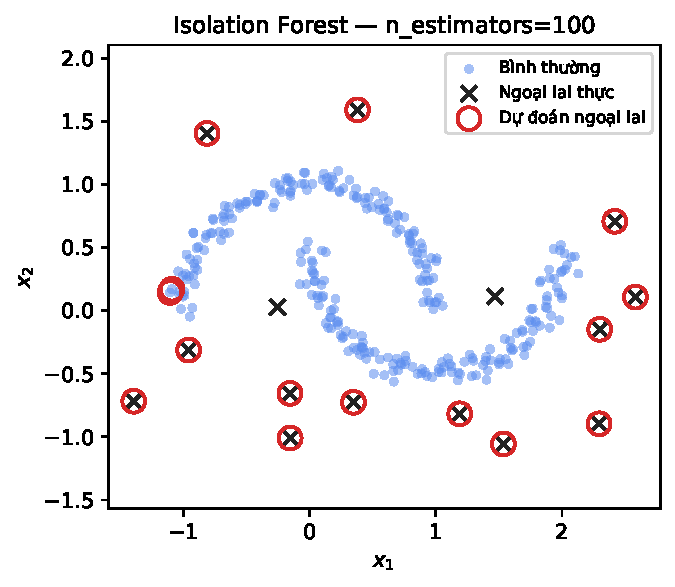
\includegraphics[width=0.55\textwidth]{iforest.pdf}
\end{center}
\noindent Trên dataset MD-NL ($n_\text{trees} = 100$, contamination $\approx 4{,}8\%$, seed $42$): phát hiện $13/15$ ngoại lai, $2$ dương tính giả, $2$ ngoại lai bị bỏ sót; $F_1 = 0{,}867$, AUC $= 0{,}993$. AUC cao cho thấy thang điểm bất thường vẫn rất phân tách; sai số chủ yếu sinh ra ở bước cắt ngưỡng theo contamination.

% --------------------------------------------------
\subsection{One-Class SVM}

\textbf{Ý tưởng.} Học một hypersphere (hoặc hyperplane) trong không gian đặc trưng bao quanh phần lớn dữ liệu huấn luyện. Các điểm nằm ngoài vùng này được coi là ngoại lai \parencite{scholkopf2001}.

\textbf{Bài toán tối ưu.} Ánh xạ dữ liệu vào không gian đặc trưng qua $\phi: \R^p \to \mathcal{H}$ với hàm nhân (kernel) $K(\mathbf{x}, \mathbf{x}') = \phi(\mathbf{x})^\top \phi(\mathbf{x}')$. Tìm siêu phẳng phân tách dữ liệu với gốc tọa độ:
\begin{equation}
  \min_{\mathbf{w},\,\boldsymbol{\xi},\,\rho} \frac{1}{2}\|\mathbf{w}\|^2 - \rho + \frac{1}{\nu n}\sum_{i=1}^n \xi_i,
  \quad \text{s.t.} \quad \mathbf{w}^\top \phi(\mathbf{x}_i) \ge \rho - \xi_i, \quad \xi_i \ge 0.
\end{equation}

Tham số $\nu \in (0, 1]$ điều chỉnh tỉ lệ ngoại lai cho phép: $\nu$ là cận trên của tỉ lệ điểm bị phân loại nhầm trong tập huấn luyện.

\textbf{Hàm quyết định.}
\begin{equation}
  f(\mathbf{x}) = \operatorname{sign}\bigl(\mathbf{w}^\top \phi(\mathbf{x}) - \rho\bigr) = \operatorname{sign}\Bigl(\sum_i \alpha_i K(\mathbf{x}_i, \mathbf{x}) - \rho\Bigr).
\end{equation}
Quan sát $\mathbf{x}$ là ngoại lai nếu $f(\mathbf{x}) = -1$.

\textbf{Hàm nhân RBF} (thường dùng): $K(\mathbf{x}, \mathbf{x}') = \exp(-\gamma\|\mathbf{x} - \mathbf{x}'\|^2)$.

\begin{lstlisting}[style=pseudo, caption={One-Class SVM}, label={lst:ocsvm}]
Input:  training data X_train, kernel K (e.g. RBF), nu, gamma
Output: decision function f, outliers O on test set X_test

// Training
alpha, rho = solve_QP(X_train, K, nu)  // quadratic programming
// alpha_i > 0 only for support vectors

// Scoring
O = []
for each x in X_test:
    score = sum(alpha_i * K(x_i, x) for i in support_vectors) - rho
    if score < 0 then O.append(x)
return f, O
\end{lstlisting}

\textbf{Nhược điểm:} tốc độ huấn luyện $O(n^2)$ đến $O(n^3)$, nhạy cảm với lựa chọn tham số $\nu$ và $\gamma$.

\noindent\textbf{Minh họa thực nghiệm.}
\begin{center}
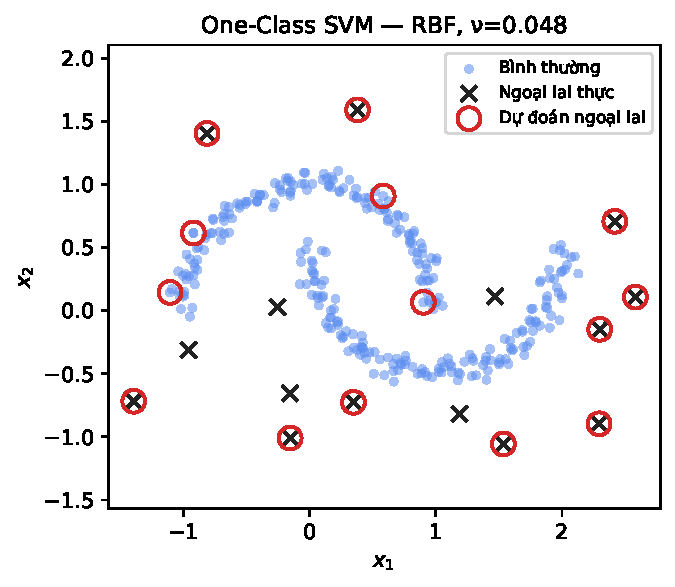
\includegraphics[width=0.55\textwidth]{ocsvm.pdf}
\end{center}
\noindent Trên dataset MD-NL (RBF, $\nu \approx 0{,}048$, $\gamma$ = 'scale', dữ liệu đã chuẩn hóa): phát hiện $10/15$ ngoại lai, $5$ dương tính giả, $5$ ngoại lai bị bỏ sót; $F_1 = 0{,}667$, AUC $= 0{,}867$. Đây là phương pháp yếu nhất trên ba phương pháp ML — biên RBF với $\gamma$ mặc định không ôm sát hai cụm half-moon, dẫn tới việc một số điểm rìa của cụm bị xếp sai loại.

% --------------------------------------------------
\subsection{Autoencoder}

\textbf{Ý tưởng.} Huấn luyện mạng nơ-ron để tái tạo lại dữ liệu đầu vào qua một cổ chai chiều thấp \parencite{sakurada2014}. Dữ liệu bình thường được tái tạo tốt; dữ liệu bất thường gây ra sai số tái tạo lớn.

\textbf{Kiến trúc.}
\begin{itemize}[noitemsep]
  \item \textbf{Bộ mã hóa (Encoder):} $\mathbf{z} = f_e(\mathbf{x};\, \theta_e)$, với $\mathbf{z} \in \R^d$, $d \ll p$.
  \item \textbf{Bộ giải mã (Decoder):} $\hat{\mathbf{x}} = f_d(\mathbf{z};\, \theta_d)$.
\end{itemize}

\textbf{Huấn luyện.} Tối thiểu hóa sai số tái tạo trên tập huấn luyện:
\begin{equation}
  \min_{\theta_e, \theta_d} \sum_{i=1}^n \|\mathbf{x}_i - f_d(f_e(\mathbf{x}_i))\|^2.
\end{equation}

\textbf{Anomaly score.}
\begin{equation}
  a(\mathbf{x}) = \|\mathbf{x} - \hat{\mathbf{x}}\|^2.
\end{equation}
Quan sát có $a(\mathbf{x})$ vượt ngưỡng $\tau$ (thường lấy từ phân vị cao của phân phối sai số trên dữ liệu xác thực) được coi là ngoại lai.

\begin{lstlisting}[style=pseudo, caption={Autoencoder cho phát hiện ngoại lai}, label={lst:ae}]
Input:  training data X_train, architecture (d_hidden, d_latent),
        epochs, contamination rate c
Output: anomaly scores, outliers O

// Training: minimize reconstruction error
model = build_AE(layers=[p, d_hidden, d_latent, d_hidden, p])
for epoch = 1 to epochs:
    for batch in X_train:
        x_hat = model.forward(batch)        // encode then decode
        loss  = mean_squared_error(batch, x_hat)
        model.backprop(loss)

// Set threshold from training errors
errors = [norm(x - model(x))^2 for x in X_train]
tau = quantile(errors, 1 - c)

// Score and flag
O = []
for each x in X_test:
    a = norm(x - model(x))^2
    if a > tau then O.append(x)
return errors, O
\end{lstlisting}

\textbf{Ứng dụng:} đặc biệt hiệu quả với dữ liệu dạng ảnh, chuỗi thời gian đa biến, và dữ liệu có cấu trúc không gian.

\noindent\textbf{Minh họa thực nghiệm.}
\begin{center}
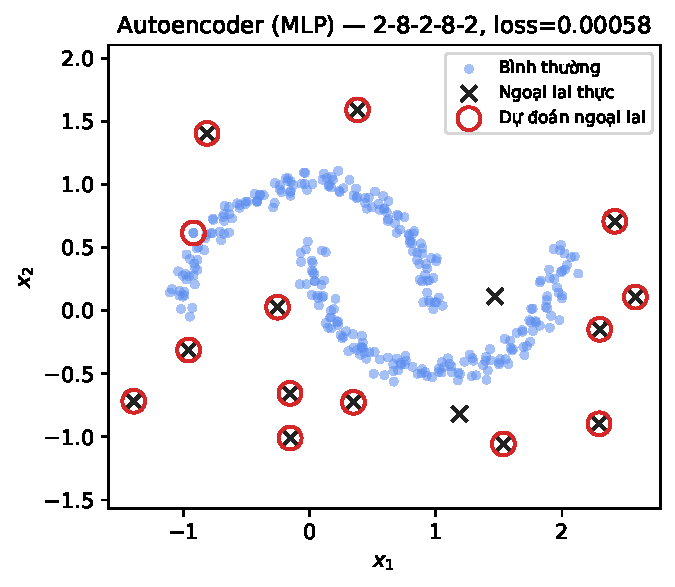
\includegraphics[width=0.55\textwidth]{autoencoder.pdf}
\end{center}
\noindent Mô phỏng autoencoder bằng \texttt{sklearn.neural\_network.MLPRegressor} với kiến trúc $2$--$8$--$2$--$8$--$2$ (cổ chai $2$ nút, kích hoạt tanh), huấn luyện target $=$ input trên dataset MD-NL: phát hiện $13/15$ ngoại lai, $2$ dương tính giả, $2$ ngoại lai bị bỏ sót; $F_1 = 0{,}867$, AUC $= 0{,}920$. Hiệu năng tương đương Isolation Forest trong khi yêu cầu nhiều tài nguyên hơn — autoencoder chỉ thực sự bộc lộ sức mạnh trên dữ liệu chiều cao và có cấu trúc.

\medskip
\noindent\textit{Lưu ý kỹ thuật.} Một \texttt{MLPRegressor} với hàm kích hoạt phi tuyến và các lớp ẩn dạng cổ chai là một autoencoder thực sự. Cách triển khai này tương đương về mặt mô hình với một autoencoder trong PyTorch/Keras, chỉ khác về API và bộ tối ưu mặc định.

% ============================================================
\section{Thí nghiệm và kết quả tổng hợp}
% ============================================================

Để định lượng hiệu năng của 11 phương pháp đã trình bày, chúng tôi tiến hành một bộ thí nghiệm tái lập được trên dữ liệu mô phỏng. Toàn bộ mã nguồn nằm trong thư mục \texttt{code/} và có thể chạy lại bằng một lệnh duy nhất \texttt{python run\_all.py}; mọi nguồn ngẫu nhiên đều được seed bằng $42$.

\subsection{Thiết lập thí nghiệm}

Ba tập dữ liệu được sinh để đại diện cho ba ngữ cảnh điển hình:

\begin{enumerate}[noitemsep, topsep=2pt]
  \item \textbf{Dataset UD --- đơn biến} ($n = 210$). 200 quan sát từ $\mathcal{N}(50, 5^2)$ và 10 ngoại lai chia đều: 5 từ $\mathcal{N}(80, 2^2)$, 5 từ $\mathcal{N}(20, 2^2)$.
  \item \textbf{Dataset MD2 --- đa biến Gaussian 2D} ($n = 215$). 200 quan sát từ $\mathcal{N}_2(\mathbf{0}, \boldsymbol{\Sigma})$ với
  $\boldsymbol{\Sigma} = \begin{psmallmatrix}2 & 1{,}5\\ 1{,}5 & 2\end{psmallmatrix}$, cộng 15 ngoại lai phân phối đều trên $[-8, 8]^2$ (chỉ giữ các điểm có $D > 5$).
  \item \textbf{Dataset MD-NL --- đa biến phi tuyến} ($n = 315$). 300 quan sát từ \texttt{make\_moons} với \texttt{noise} $= 0{,}05$, cộng 15 ngoại lai phân phối đều quanh hộp bao quan sát.
\end{enumerate}

\begin{center}
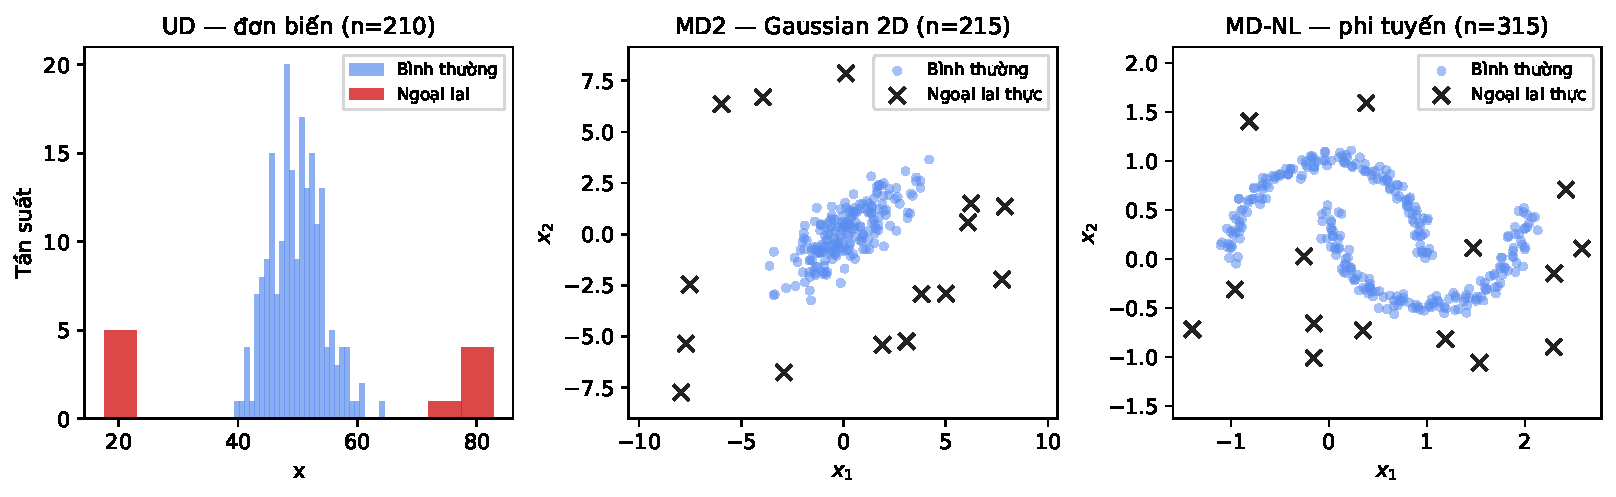
\includegraphics[width=\textwidth]{dataset_overview.pdf}\\
\captionof{figure}{Tổng quan ba tập dữ liệu mô phỏng dùng trong thí nghiệm.}
\label{fig:dataset-overview}
\end{center}

Mỗi phương pháp đơn biến được áp dụng cho UD; Mahalanobis và PCA cho MD2; còn DBSCAN, LOF, Isolation Forest, One-Class SVM và Autoencoder cho MD-NL. Đối với các phương pháp cần biết tỉ lệ ngoại lai, chúng tôi đặt \texttt{contamination} $= 15/315 \approx 0{,}048$ để khớp với tỉ lệ thực tế. Tham số khác giữ nguyên giá trị được đề xuất trong phần lý thuyết của từng phương pháp.

\subsection{Bảng metric tổng hợp}

Bảng~\ref{tab:experiment-results} tóm tắt số TP/FP/FN cùng các chỉ số Precision, Recall, F1 và ROC-AUC. ROC-AUC được tính trên thang điểm liên tục mà mỗi phương pháp xuất ra (xem mã nguồn \texttt{evaluate.py}); với DBSCAN, chúng tôi dùng khoảng cách trung bình tới $5$ lân cận gần nhất làm điểm số đại diện.

% Bảng được sinh tự động từ code/run_all.py — KHÔNG sửa tay.
\begin{table}[ht]
\centering
\caption{Kết quả thực nghiệm của 11 phương pháp trên 3 dataset mô phỏng (seed = 42).}
\label{tab:experiment-results}
\small
\begin{tabular}{llccccccc}
\toprule
\textbf{Phương pháp} & \textbf{Dataset} & \textbf{TP} & \textbf{FP} & \textbf{FN} & \textbf{Precision} & \textbf{Recall} & \textbf{F1} & \textbf{AUC} \\
\midrule
Z-score & UD & 10 & 0 & 0 & 1,000 & 1,000 & 1,000 & 1,000 \\
Modified Z-score & UD & 10 & 0 & 0 & 1,000 & 1,000 & 1,000 & 1,000 \\
IQR (Tukey) & UD & 10 & 1 & 0 & 0,909 & 1,000 & 0,952 & 1,000 \\
Grubbs (ESD) & UD & 10 & 0 & 0 & 1,000 & 1,000 & 1,000 & 1,000 \\
Mahalanobis & MD2 & 15 & 0 & 0 & 1,000 & 1,000 & 1,000 & 1,000 \\
PCA (T$^2$, Q) & MD2 & 15 & 2 & 0 & 0,882 & 1,000 & 0,938 & 1,000 \\
DBSCAN & MD-NL & 15 & 0 & 0 & 1,000 & 1,000 & 1,000 & 1,000 \\
LOF & MD-NL & 15 & 0 & 0 & 1,000 & 1,000 & 1,000 & 1,000 \\
Isolation Forest & MD-NL & 13 & 2 & 2 & 0,867 & 0,867 & 0,867 & 0,993 \\
One-Class SVM & MD-NL & 10 & 5 & 5 & 0,667 & 0,667 & 0,667 & 0,867 \\
Autoencoder (MLP) & MD-NL & 13 & 2 & 2 & 0,867 & 0,867 & 0,867 & 0,920 \\
\bottomrule
\end{tabular}
\medskip

\textit{Ghi chú}: TP = số ngoại lai phát hiện đúng; FP = số điểm bình thường bị gắn nhầm là ngoại lai; FN = số ngoại lai bị bỏ sót. Mỗi dataset có số ngoại lai thực: UD = 10, MD2 = 15, MD-NL = 15.
\end{table}


\subsection{So sánh trực quan}

Hình~\ref{fig:score-comparison} biểu diễn cùng kết quả dưới dạng biểu đồ thanh, giúp dễ đối chiếu giữa các phương pháp.

\begin{center}
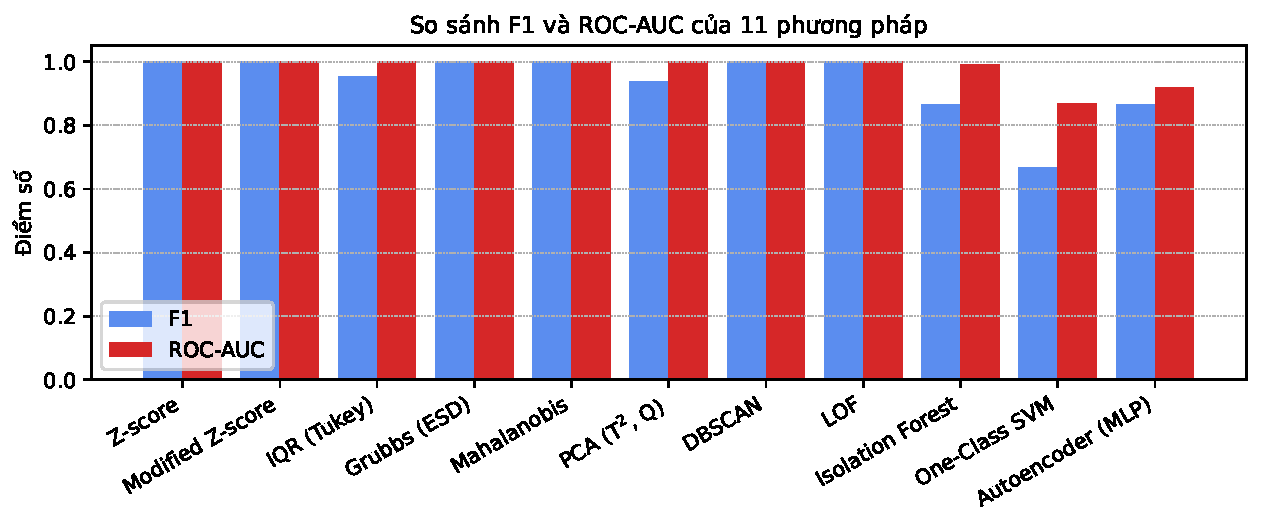
\includegraphics[width=\textwidth]{score_comparison.pdf}\\
\captionof{figure}{So sánh F1 và ROC-AUC giữa 11 phương pháp.}
\label{fig:score-comparison}
\end{center}

\subsection{Thảo luận}

\paragraph{Trên dataset UD.} Tất cả bốn phương pháp đơn biến đều phát hiện đầy đủ 10 ngoại lai vì khoảng cách giữa chúng và phân phối nội tại (cách trung bình khoảng $6\sigma$) đủ lớn. Tuy vậy, IQR sinh thêm $1$ dương tính giả ngay tại rìa hàng rào trong --- một phản ứng đặc trưng của hệ số $1{,}5$. Điều này phù hợp với kỳ vọng lý thuyết: trong điều kiện \emph{ngoại lai rất rõ ràng và mẫu lớn}, hiệu ứng masking của Z-score chưa đủ trọng số để làm hỏng kết quả. Với mẫu nhỏ hơn hoặc ngoại lai gần ngưỡng, lợi thế của Modified Z-score và Grubbs ESD sẽ rõ rệt hơn.

\paragraph{Trên dataset MD2.} Mahalanobis đạt $F_1 = 1{,}000$, phản ánh đúng môi trường lý tưởng cho phương pháp: dữ liệu Gaussian, ngoại lai rời xa cụm chính. PCA $T^2$/$Q$ phát hiện đầy đủ ngoại lai (Recall $= 1$) nhưng kèm $2$ dương tính giả; điều này đến từ việc với $p = 2$ và chọn $k = 1$, không gian \emph{residual} chỉ còn một chiều, nên ngưỡng Jackson--Mudholkar trở nên hơi chặt. Trên dữ liệu nhiều chiều thực sự, PCA thường vượt trội Mahalanobis nhờ giảm chiều và giảm tác động của hiệp phương sai gần suy biến.

\paragraph{Trên dataset MD-NL.} DBSCAN và LOF đạt phân tách hoàn hảo nhờ tính chất \emph{cục bộ}: chúng không cần giả định cụm có hình dạng lồi. Đáng chú ý, Mahalanobis nếu áp dụng tại đây sẽ thất bại vì hai cụm half-moon có tâm gần nhau nhưng phương sai lớn, biến đa số các ngoại lai uniform thành điểm ``trong vùng tin cậy'' của một $\boldsymbol{\Sigma}$ phồng. Trong nhóm ML, Isolation Forest và Autoencoder đạt $F_1 = 0{,}867$ với AUC lần lượt $0{,}993$ và $0{,}920$, cho thấy thang điểm \emph{thực sự} phân tách tốt --- sai số chủ yếu sinh ra ở bước cắt ngưỡng theo \texttt{contamination}. One-Class SVM với $\gamma$ mặc định ('scale') không ôm sát được hai cụm half-moon, dẫn tới $F_1 = 0{,}667$, AUC $= 0{,}867$, là phương pháp yếu nhất trong nhóm này.

\paragraph{Hệ quả thực tiễn.} Kết quả tái khẳng định ba thông điệp đã quen thuộc trong cộng đồng phân tích dữ liệu: (i) chọn phương pháp phải đồng bộ với cấu trúc dữ liệu --- không có ``công cụ tốt nhất'' cho mọi tình huống; (ii) các phương pháp đơn giản (IQR, Modified Z-score, Mahalanobis) là baseline mạnh và nên thử trước; (iii) khi dữ liệu có cấu trúc cụm phi tuyến, các phương pháp dựa trên mật độ cục bộ (LOF, DBSCAN) thường vượt trội các phương pháp tham số cũng như các phương pháp ML không tinh chỉnh kỹ siêu tham số.

% ============================================================
\section{So sánh và hướng dẫn lựa chọn phương pháp}
% ============================================================

Bảng~\ref{tab:comparison} tổng hợp các đặc điểm chính của từng phương pháp.

\begin{table}[ht]
\centering
\caption{So sánh các phương pháp phát hiện điểm ngoại lai (TN = thực nghiệm trên dataset tương ứng)}
\label{tab:comparison}
\footnotesize
\begin{tabular}{llllccc}
\toprule
\textbf{Phương pháp} & \textbf{Phạm vi} & \textbf{Giả định} & \textbf{Độ phức tạp} & \textbf{Robust} & \textbf{F1 (TN)} & \textbf{AUC (TN)} \\
\midrule
Z-score             & Đơn biến & Gaussian      & $O(n)$                & Không & 1,000 & 1,000 \\
Modified Z-score    & Đơn biến & Gaussian yếu  & $O(n \log n)$         & Có    & 1,000 & 1,000 \\
IQR                 & Đơn biến & Không có      & $O(n \log n)$         & Có    & 0,952 & 1,000 \\
Kiểm định Grubbs   & Đơn biến & Gaussian      & $O(n^2)$              & Không & 1,000 & 1,000 \\
\midrule
Mahalanobis         & Đa biến  & Gaussian      & $O(np^2 + p^3)$       & Không$^*$ & 1,000 & 1,000 \\
PCA ($T^2$, $Q$)   & Đa biến  & Gaussian      & $O(np^2)$             & Không & 0,938 & 1,000 \\
\midrule
DBSCAN              & Đa biến  & Không có      & $O(n \log n)$         & Có    & 1,000 & 1,000 \\
LOF                 & Đa biến  & Không có      & $O(n^2)$              & Có    & 1,000 & 1,000 \\
\midrule
Isolation Forest    & Đa biến  & Không có      & $O(t\psi \log\psi)$   & Có    & 0,867 & 0,993 \\
One-Class SVM       & Đa biến  & Không có      & $O(n^2)$--$O(n^3)$    & Có    & 0,667 & 0,867 \\
Autoencoder         & Đa biến  & Không có      & phụ thuộc kiến trúc   & Có    & 0,867 & 0,920 \\
\bottomrule
\multicolumn{7}{l}{\footnotesize $^*$ Robust nếu dùng ước lượng MCD \parencite{rousseeuw1999} thay vì hiệp phương sai mẫu.}
\end{tabular}
\end{table}

\subsection{Hướng dẫn lựa chọn}
Căn cứ vào đặc điểm bài toán, người thực hành có thể tham khảo các gợi ý sau:

\begin{enumerate}[noitemsep]
  \item \textbf{Dữ liệu đơn biến, phân phối Gaussian, mẫu nhỏ:} Kiểm định Grubbs cho kiểm soát mức ý nghĩa chính xác; Z-score cho tốc độ.
  \item \textbf{Dữ liệu đơn biến, phân phối không rõ:} IQR hoặc Modified Z-score --- không tham số, robust.
  \item \textbf{Dữ liệu đa biến tuyến tính, phân phối Gaussian:} Khoảng cách Mahalanobis (với MCD nếu cần robustness); PCA nếu muốn hiểu cấu trúc phương sai.
  \item \textbf{Dữ liệu có cụm hình dạng tùy ý:} DBSCAN (phân cụm kết hợp) hoặc LOF (điểm số liên tục).
  \item \textbf{Dữ liệu lớn, nhiều chiều, không có giả định phân phối:} Isolation Forest --- nhanh, hiệu quả bộ nhớ, không cần tính khoảng cách.
  \item \textbf{Dữ liệu có cấu trúc phức tạp (ảnh, chuỗi thời gian):} Autoencoder --- học biểu diễn tiềm ẩn và phát hiện dựa trên sai số tái tạo.
\end{enumerate}

% ============================================================
\section{Kết luận}
% ============================================================

Bài báo cáo đã trình bày một bức tranh tổng quan về các phương pháp phát hiện điểm ngoại lai, từ các kiểm định thống kê cổ điển (Z-score, IQR, Grubbs) qua các phương pháp đa biến (Mahalanobis, PCA) và dựa trên mật độ (DBSCAN, LOF) đến các phương pháp học máy hiện đại (Isolation Forest, One-Class SVM, Autoencoder).

Không tồn tại một phương pháp tối ưu cho mọi tình huống. Lựa chọn phụ thuộc vào:
số chiều của dữ liệu, giả định về phân phối, nhu cầu về khả năng giải thích, quy mô dữ liệu, và tỉ lệ ngoại lai dự kiến.
Trong thực tiễn, thường kết hợp nhiều phương pháp và xác nhận kết quả bằng kiến thức chuyên ngành (domain knowledge).

Các hướng nghiên cứu hiện đại bao gồm: phát hiện ngoại lai theo luồng thời gian thực (\textit{streaming anomaly detection}), phương pháp sâu dựa trên mô hình sinh (\textit{VAE}, \textit{GAN}), và giải thích điểm ngoại lai (\textit{explainable anomaly detection}).

% ============================================================
\printbibliography[title={Tài liệu tham khảo}]
% ============================================================

\end{document}
